\documentclass{beamer}
\usepackage[spanish]{babel}
\usepackage[utf8]{inputenc}
\usepackage{multicol} % indice en 2 columnas
\usepackage{graphicx}
\usepackage{enumitem}
\usepackage{xcolor}

%configura la figura de las listas itemize
\setlist[itemize]{label={\color{blue}$\bullet$}}
\usetheme{Warsaw}
\usecolortheme{dolphin}
\useoutertheme{shadow}
\useinnertheme{rectangles}

% 1º ppt
\title[IPv6]{Migrando aplicaciones a IPv6}
\subtitle{Estado actual y fundamentos de nuestro proyecto}
\author[Sandoval, Vargas]
{Alonso Sandoval A. \and Hernán Vargas L.}
\institute[UTFSM]
{
  Universidad Técnica Federico Santa María
  \and
  \texttt{asandova@alumnos.inf.utfsm.cl, hvargas@alumnos.inf.utfsm.cl}
}
\date{\today}

%2º ppt
\AtBeginSection{
\begin{frame}
  \frametitle{Índice}
  \tableofcontents[currentsection]   
\end{frame}
}

\AtBeginSubsection{
\begin{frame}
  \frametitle{Índice}
  \tableofcontents[currentsection,currentsubsection]
\end{frame}
}

\begin{document}

\frame{\titlepage}

\begin{frame}
  \frametitle{Índice}
  \tableofcontents
\end{frame}

\section{Contexto protocolo de internet}
\subsection{Problemática actual}

\begin{frame}
  \frametitle{Problemática direcciones IPv4}
	\begin{itemize}
		\item
			La cantidad de direcciones IPv4 no dan a vasto:
			$4\cdot10^{9}$ app.\bigskip
		\item
			La solución al problema consiste en la 
			implementación de IPv6, con una cantidad
			de direcciones:
			$3,40\cdot10^{38}$ app.\bigskip
		\item
			Lamentablemente, IPv6 e IPv4 no son
			compatibles.
	\end{itemize}
% Mini bloques dentro de las ppt
%\begin{block}{Marsupiales en Australia}
% Koala, Canguro, Wombat...
%\end{block}       
\end{frame}

\subsection{IPv6 vs IPv4}

\begin{frame}
  \frametitle{Comparación cabeceras}
  \begin{columns}[t]
    \column{0.5\textwidth}
    	\begin{figure}
		\centering
		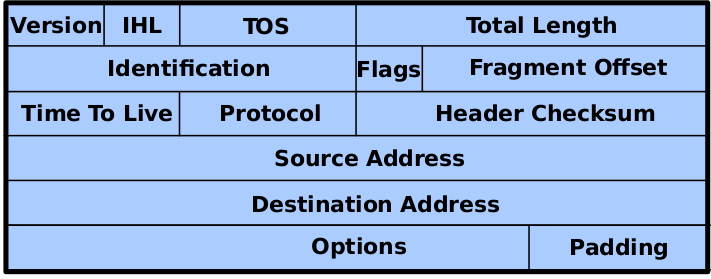
\includegraphics[width=150px]{img/ipv4_cab.png}
		\caption{IPv4}
	\end{figure}
    \column{0.5\textwidth}
	 \begin{itemize}
		\tiny 
		\item
			Version: Versión protocolo, 4.
		\item
			IHL: Tamaño encabezado IP
		\item
			TOS: Calidad de Servicio. Priorización paquetes.
		\item
			Total Length: Tamaño total datagrama, carga útil.
		\item
			Identification: Identificador para re-ensamblado
		\item
			Flags: Bits de control sobre la fragmentación
		\item
			Fragment Offset: Ubicación de este fragmento dentro
			del datagrama original
		\item
			TTL: Tiempo máximo vida datagrama.
		\item
			Protocol: Protocolo carga útil del paquete IP
		\item
			Header Checksum: Suma comprobación de paquetes
		\item
			Options: Campo opcionales, rara vez utilizado.
		\item
			Padding: Relleno con ceros, asegura que
			encabezado sea de tamaño múltiplo de 32 bits.
	 \end{itemize}
  \end{columns}
\end{frame}

\begin{frame}
  \frametitle{Comparación cabeceras}
  \begin{columns}[t]
    \column{0.5\textwidth}
    	\begin{figure}
		\centering
		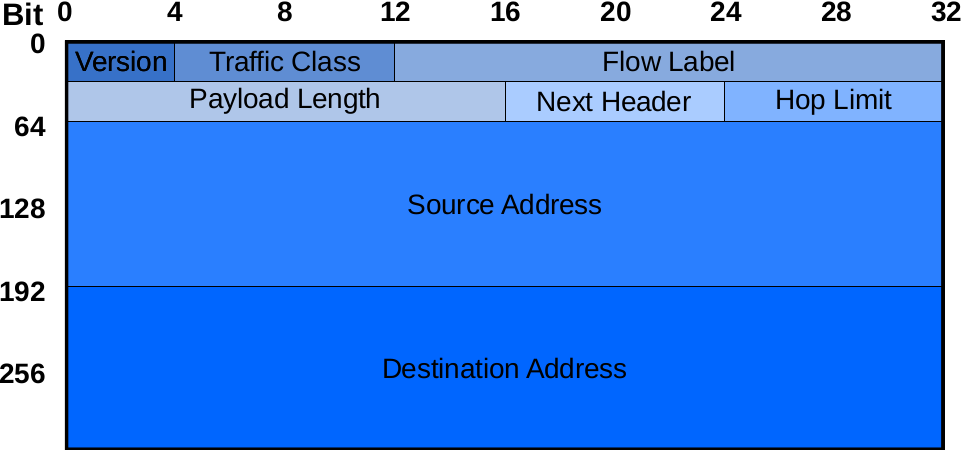
\includegraphics[width=125px]{img/ipv6_cab.png}
		\caption{IPv6}
	\end{figure}
    \column{0.5\textwidth}
    	\begin{itemize}
		\small
		\item
			Version: Versión protocolo, 6.
		\item
			Traffic Class: Implementación Calidad servicio.
		\item
			Flow Label: Permite definición flujo de datos.
		\item
			Payload Length: Tamaño carga útil.
		\item
			Next Header: Tipo de encabezado que está a 
			continuación del encabezado IPv6
		\item
			Hop LImit: Cantidad máxima saltos permitidos.
	\end{itemize}
  \end{columns}
\end{frame}
\begin{frame}
  \frametitle{Comparación cabeceras}
  Cabe agregar que el campo opciones se deja como encabezado de extensión,
  con las posibles opciones:
  \begin{itemize}
	\item
		Hop-by-Hop Options: Opciones a revisar en cada salto.
	\item
		Routing: Especifica nodos intermedios a visitar antes
		de llegar a destino.
	\item
		Fragment: Utilizado apra fragmentar paquetes con tamaño 
		superior al MTU de algún enlace.
	\item
		Destination Options: Opciones revisadas por nodo de 
		destino.
	\item
		Authentication: Para servicio de autenticación (IPsec)
	\item
		Encapsulating Security Payload: Diseñado para
		proveer confidencialidad, autenticación de origen, 
		integridad, otros.
  \end{itemize}
\end{frame}
\begin{frame}
  \frametitle{Algunas mejoras y diferencias de IPv6 con IPv4}
  \begin{itemize}
	\item
		Formato Decimal a Hexadecimal: 
		IPv4: 192.168.1.1, IPv6: 2001:0DB8:0:0:0:0:0:003D.
	\item
		Multicast Reemplaza a Broadcast: Mensajes múltiples
		a destinos específicos.
	\item
		Autoconfiguracion de direcciones: Neighbor Discovery
		Protocol.
	\item
		Capa Seguridad: IPsec, uso en seguridad.
	\item
		Procesamiento simplificado: Eliminación de campos
		encabezado IPv6.
	\item
		Extensiones de Privacidad: Permite que
		direcciones auto-asignadas  cambien con el tiempo.
  \end{itemize}
\end{frame}

%more...

\subsection{Principales implementaciones de IPv6}
\begin{frame}
	\frametitle{IPv6 sobre IPv4 (Máquinas IPv4 en internet IPv6)}
	\begin{itemize}[itemsep=2em]
		\item
			6to4: A través de un túnel (Tunnel Broker),
			permite salida a internet IPv4 desde red IPv6.
		\item
			6in4: Paso de paquetes IPv6 como payload de IPv4.
		\item
			6over4: Requiere uso de multicast, no soportado
			ampliamente por IPv4.
		\item
			6rd: similar a 6to4 solo que el ISP provee del 
			Tunnel Broker.
	\end{itemize}
\end{frame}

\begin{frame}
	\frametitle{IPv4 sobre IPv6 (No muy usado)}
	\begin{itemize}[itemsep=3em]
		\item
			Nat64/DNS64: DNS especial hace la traducción
			de registros A(IPv4) con quad A (IPv6).
		\item
			4in6: Paquete IPv4 en en contenido de paquete IPv6.
		\item
			4rd: Opuesto a 6rd
	\end{itemize}
\end{frame}
\begin{frame}
\frametitle{Dual Stack}
	\begin{itemize}
		\item
			El método ideal ya que permite acceso
			nativo a ambos protocolos (Ipv4 e IPv6) de manera 
			simultánea
			evitando costos en infraestructura(túneles por 
			ejemplo) remitiendo
			estos a la adquisición de hadware.
	\end{itemize}
	\begin{figure}
		\centering
		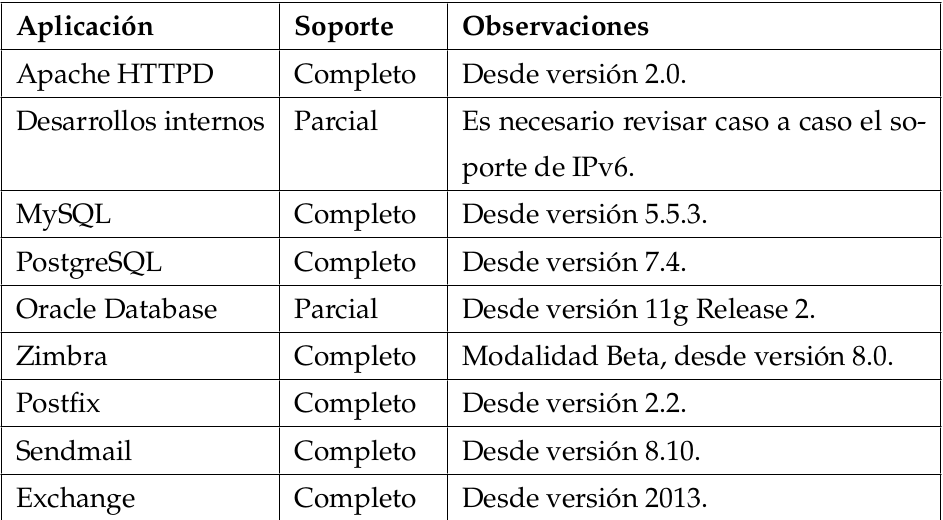
\includegraphics[width=200px]{img/apps.png}
	\end{figure}
\end{frame}


\section{Proyecto aplicación Dual Stack}

%tex_origin: ppt.tex
\subsection{Idea}
\begin{frame}
	\frametitle{Aplicación}
	\begin{itemize}
	\item
		Dos aplicaciones conectadas por sockets, una para el cliente y otra
		para el servidor.
	\item
		El servidor es capaz de aplicar dual-stack, es decir, procesa los
		paquetes sin importar si vienen en IPv4 o IPv6.
	\item
		El cliente es capaz de enviar paquetes de ambos protocolos.
	\item
		Se pueden obtener estadísticas de las operaciones efectuadas (tiempos,
		tazas de perdida, entre otros).
	\end{itemize}
\end{frame}

\begin{frame}
	\frametitle{Aplicación}
	\begin{figure}
		\centering
		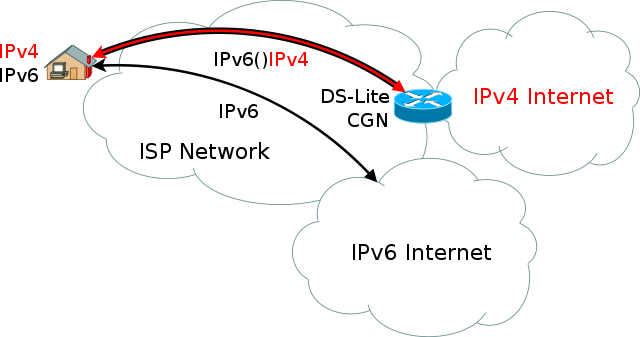
\includegraphics[width=300px]{img/dualstack.png}
	\end{figure}
\end{frame}


\subsection{Entorno de desarrollo}

\begin{frame}
  \frametitle{Internet IPv6}
  \begin{itemize}[itemsep=3em]
  \item
	  La mayoría de los ISP no proveen de acceso a la red IPv6 en
	  los hogares.
  \item
	  El departamento de Informática de la UTFSM ofrece el acceso
	  a la red local en IPv6
  \item
	  Por ello, utilizaremos una máquina virtual en la red del DI
	  como servidor con la cual nos comunicaremos en la misma
	  red bajo IPv6.
  \end{itemize}
\end{frame}

\begin{frame}
  \frametitle{Máquina virtual}
  \begin{itemize}[itemsep=3em]
  \item
	  Utilizaremos una VM que nos disponga algún laboratorio
	  en el departamento.
  \item
	  Para la VM utilizaremos la distribución de linux CentOS
	  que soporta IPv6 además de estar orientada a servidores.
	\begin{figure}
		\centering
		
\includegraphics[width=200px]{img/centos.png}
	\end{figure}
  \end{itemize}
\end{frame}

%tex_origin: ppt.tex
\subsection{Sockets.h}
\begin{frame}
  \frametitle{Sockets}
  \begin{itemize}
  \item	
	  Un socket es un mecanismo por el cual se traspasan mensajes entre
	  aplicaciones, generalmente en diferentes computadores.
  \item	
	  Está definido al menos por las direcciones IP, números de puerto y el 
	  protocolo de transporte.
  \item
	  Los protocolos más utilizados son TCP y UDP.
  \item
	  Implementan la arquitectura cliente-servidor, el programa que inicia la 
	  comunicación será el cliente, mientras que el que responde actúa como
	  servidor.
  \end{itemize}
\end{frame}

\begin{frame}
  \frametitle{socket.h}
  \begin{itemize}
  \item	
	  API para el trabajo con sockets en c para linux.
  \item
	  Soporta tanto IPv4 como IPv6.
  \item
	  Incorpora funciones para la creación de sockets, convención entre
	  formatos, y transmisión de datos.
  \item
	  Define estructuras para el manejo de direcciones.
  \end{itemize}
\end{frame}

\begin{frame}
	\frametitle{socket.h (continuación)}
	En general el procedimiento es el siguiente:
	\begin{itemize}
		\item
			Se crea la estructura para manejar la dirección.
			\texttt{sockaddr\_in} para IPv4 y \texttt{sockaddr\_in6} para IPv6.
		\item
			Se crea el socket y se le asigna un descriptor.
			\texttt{socket();}
		\item
			Se asocia el socket y la estructura de dirección. \texttt{bind();} 
		\item
			Se pone al socket como ``escucha'' esperando conexiones.
			\texttt{accept();}
		\item
			Cuando una conexión es detectada se crea un nuevo socket, al que se
			le llama ``socket conectado''.
		\item
			Se puede lanzar un subproceso para continuar ``escuchando'' y 
			trabajar con el ``socket conectado''.
	\end{itemize}
\end{frame}
			
\frame{\titlepage}

  
\end{document}
